\thispagestyle{timhieukhoahocnone}
\pagestyle{timhieukhoahoc}
\everymath{\color{timhieukhoahoc}}
\blfootnote{\color{cackithi}$^*$Đại học Osnabrueck, CHLB Đức.}
\graphicspath{{../timhieukhoahoc/pic/}}
\begingroup
\AddToShipoutPicture*{\put(0,616){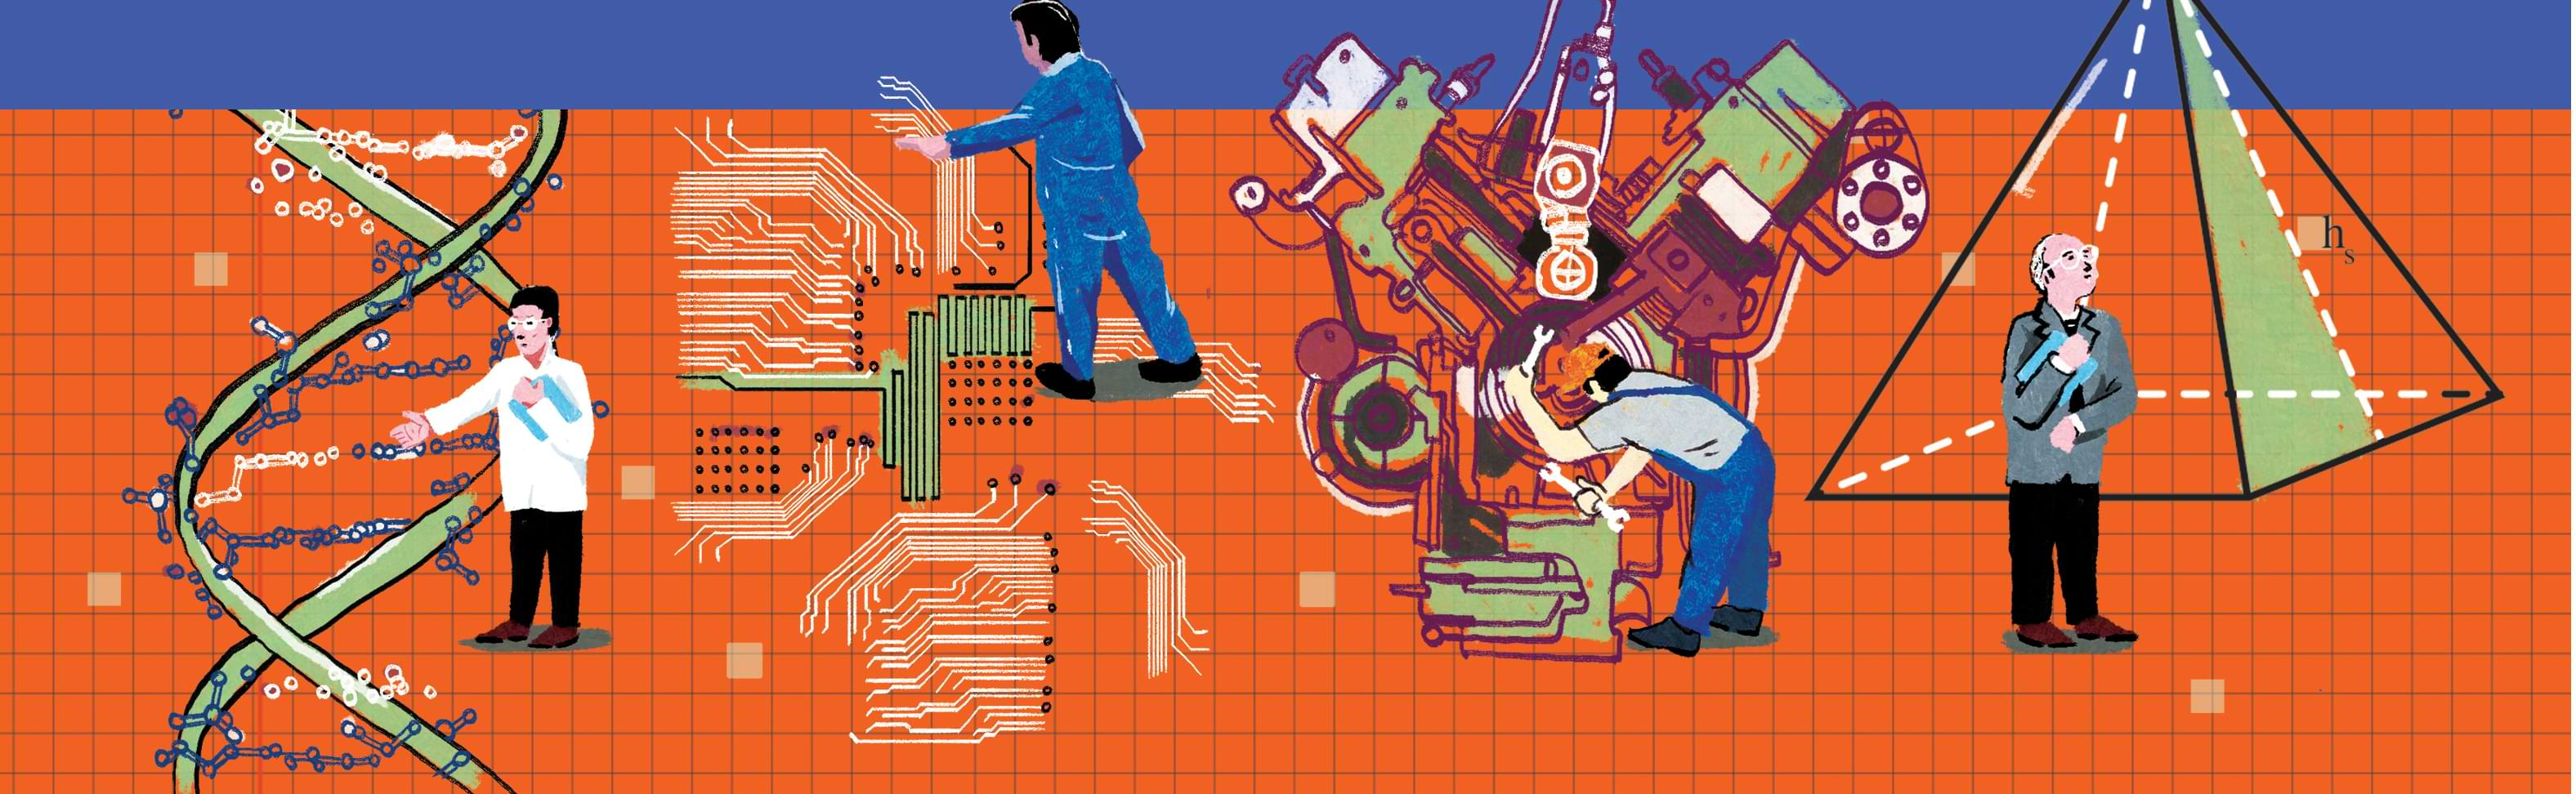
\includegraphics[width=19.3cm]{../bannertimhieu}}}
\AddToShipoutPicture*{\put(76,555){
\includegraphics[scale=1]{../tieude2.pdf}}}
\centering
\endgroup
\vspace*{155pt}



\begin{multicols}{2}
	Bất chấp lịch sử ngắn ngủi của mình, máy tính và trí tuệ nhân tạo (AI) đã thay đổi một cách cơ bản những gì chúng ta thấy, những gì chúng ta biết và những gì chúng ta làm. Chỉ trong một thời gian ngắn, các hệ thống AI đã xâm nhập vào mọi lĩnh vực của cuộc sống, từ khái quát như học tập, lý luận, nhận thức, v.v., cho đến cụ thể như chơi cờ, chứng minh các định lý toán học, vẽ tranh, sáng tác nhạc, viết tiểu luận, làm thơ, lái xe ô tô hay chẩn đoán bệnh. Thế giới thay đổi nhanh chóng đến nỗi ngay cả những công nghệ khá gần đây cũng khiến chúng ta cảm thấy lạc hậu như thế nào. Điện thoại di động vào những năm $90$ là những viên gạch lớn với màn hình nhỏ màu xanh lá cây. Hai thập kỷ trước đó, bộ lưu trữ chính của máy tính là thẻ đục lỗ.
	\begin{figure}[H]
		\vspace*{-5pt}
		\centering
		\captionsetup{labelformat= empty, justification=centering}
		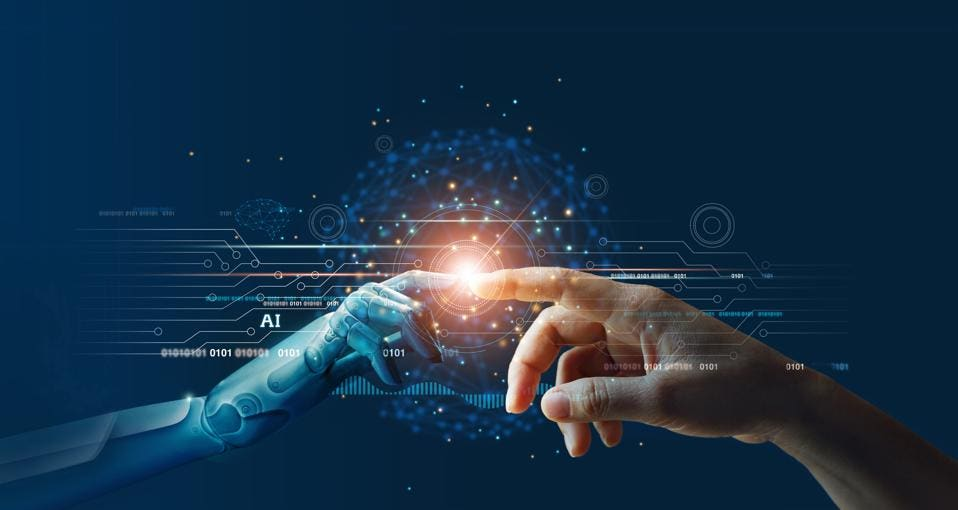
\includegraphics[width= 1\linewidth]{AI1.jpg}
		%		\caption{\small\textit{\color{}}}
		\vspace*{-15pt}
	\end{figure}
	Máy tính cùng các ứng dụng thông minh phát triển một cách nhanh chóng và trở thành một phần không thể thiếu trong cuộc sống hàng ngày của chúng ta khiến con người dễ dàng quên mất các công nghệ này mới ra đời như thế nào. Để biết tương lai sẽ ra sao, việc nghiên cứu lịch sử thường rất hữu ích. Trong bài viết này, chúng ta hãy cùng nhìn lại một số cột mốc quan trọng trong lịch sử phát triển của máy tính và lĩnh vực AI, để xem chúng ta có thể mong đợi điều gì từ chúng trong tương lai, để xem liệu AI sẽ đi đến đâu, và quan trọng hơn, nó sẽ dẫn chúng ta đến đâu.
	\vskip 0.1cm
	\textbf{\color{cackithi}Những hạt giống đầu tiên}
	\vskip 0.1cm
	Chúng ta tự gọi mình là \textit{Homo sapiens} -- con người thông thái -- bởi vì trí thông minh rất quan trọng đối với chúng ta. Trong hàng nghìn năm, chúng ta đã cố gắng hiểu cách chúng ta suy nghĩ và hành động -- nghĩa là làm thế nào bộ não của chúng ta, chỉ là một số ít vật chất, lại có thể nhận thức, hiểu, dự đoán và điều khiển một thế giới rộng lớn và phức tạp hơn chính nó rất nhiều. Từ thời cổ đại, những huyền thoại và truyền thuyết về những sinh vật nhân tạo được ban cho ý thức hoặc trí thông minh bởi những người thợ bậc thầy đã xuất hiện và được lưu truyền. Đến thế kỷ $19$ và nửa đầu thế kỷ $20$, ý tưởng về con người nhân tạo và những cỗ máy biết suy nghĩ cũng được phát triển trong các tác phẩm văn học, điển hình như quái vật Monster có sức mạnh phi thường nhưng ý thức được sự cô đơn của mình trong \textit{Frankenstein} của Mary Shelley, hay anh chàng người thiếc Woodman luôn khao khát có một trái tim trong \textit{Phù thủy xứ Oz} của Frank Baum.
	\begin{figure}[H]
		\vspace*{-5pt}
		\centering
		\captionsetup{labelformat= empty, justification=centering}
		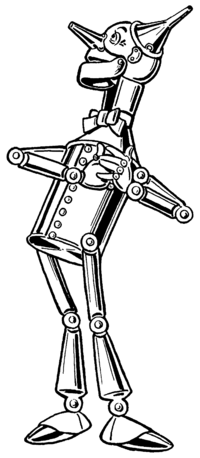
\includegraphics[width= 0.4\linewidth]{Tin_Woodman.png}
		\caption{\small\textit{\color{cackithi}Hình $1$: Phác họa của Tin Woodman. Nguồn: Wiki.}}
		\vspace*{-10pt}
	\end{figure}
	Ở khía cạnh khác, các nhà triết học qua hàng thế kỷ đã cố gắng mô tả quá trình suy nghĩ của con người như sự thao tác của các biểu tượng (ký tự). Công trình này đạt đến đỉnh cao với việc phát minh ra máy tính kỹ thuật số có thể lập trình vào những năm $1940$, một cỗ máy dựa trên bản chất trừu tượng của suy luận toán học. 
	\vskip 0.1cm
	Máy tính điện tử và những ý tưởng đằng sau nó đã truyền cảm hứng cho một số nhà khoa học đến từ nhiều lĩnh vực khác nhau (toán học, tâm lý học, kỹ thuật, kinh tế và khoa học chính trị), và họ bắt đầu thảo luận nghiêm túc về khả năng xây dựng  bộ não điện tử -- một bộ não nhân tạo có khả năng suy nghĩ và suy luận giống như bộ não của con người.
	\vskip 0.1cm
	\textbf{\color{cackithi}Bài kiểm tra Turing}
	\vskip 0.1cm
	Năm $1950$, nhà toán học kiệt xuất người Anh Alan Turing -- một trong những cha đẻ của máy tính hiện đại -- đã thảo luận về cách chế tạo những cỗ máy thông minh và để xuất một phương pháp để kiểm tra trí thông minh của chúng. Trong công trình nổi tiếng \textit{Computing machinery and
		intelligence} (Máy tính và trí thông minh), ông xem xét câu hỏi \textit{``Máy móc có thể suy nghĩ được không?"}. Turing cho rằng vì các từ ``suy nghĩ" và ``máy móc" không thể được định nghĩa rõ ràng nên chúng ta có thể thay thế câu hỏi trên bằng một câu hỏi khác, có liên quan chặt chẽ với nó, được diễn đạt bằng những từ tương đối rõ ràng và có thể kiểm chứng, chẳng hạn \textit{``Liệu \textbf{\color{cackithi}máy tính điện tử} có thể \textbf{\color{cackithi}làm} những điều mà chúng ta (những thực thể có trí tuệ) có thể làm?"}.
	\begin{figure}[H]
		\vspace*{-5pt}
		\centering
		\captionsetup{labelformat= empty, justification=centering}
		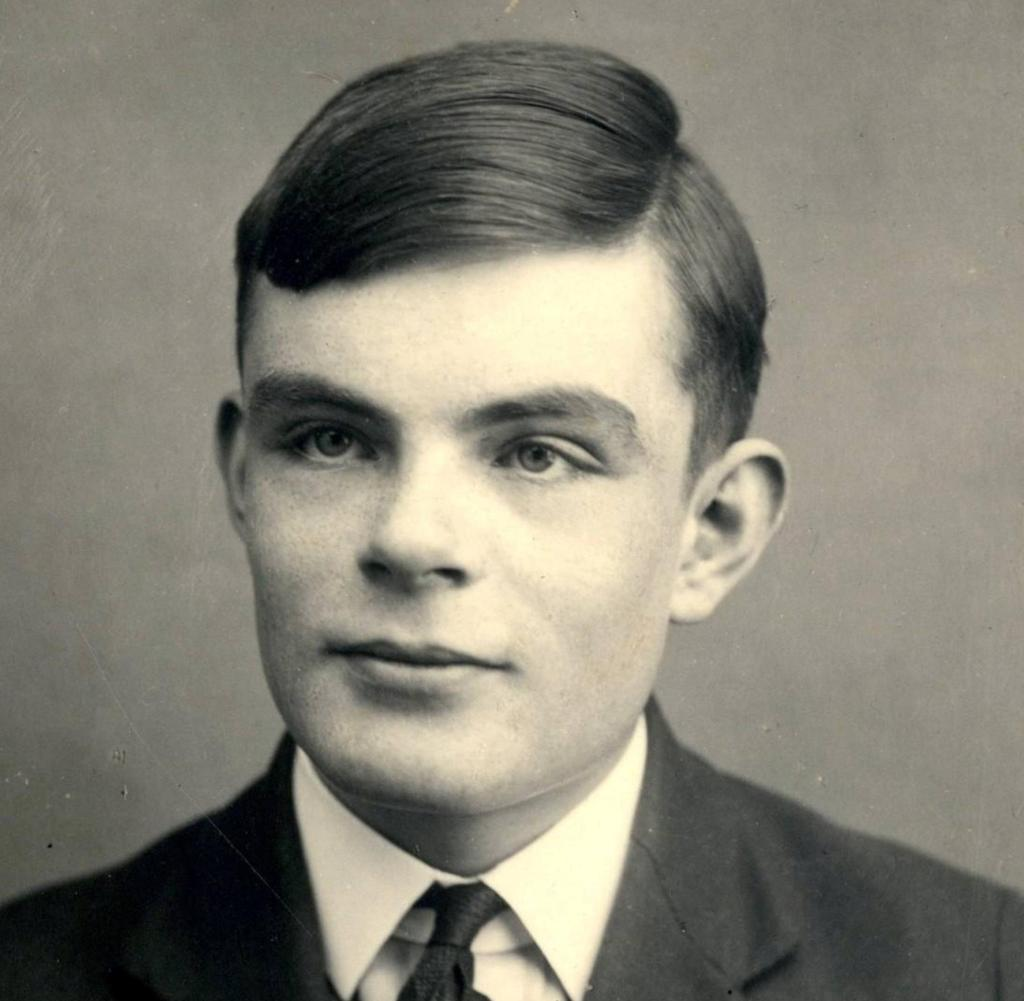
\includegraphics[width= 1\linewidth]{Alan-Turing.jpg}
		\caption{\small\textit{\color{cackithi}Hình $2$: Alan Turing. Nguồn: AFP/Getty Images.}}
		\vspace*{-10pt}
	\end{figure}
	Để trả lời cho câu hỏi trên, Turing đề xuất một phương pháp gọi là ``Trò chơi bắt chước" (Imitation game), sau này được biết đến rộng rãi với tên gọi \textit{Bài kiểm tra Turing}. Bài kiểm tra có sự tham gia của ba thành viên được xếp vào ba căn phòng tách biệt: Một người thẩm vấn (C), một máy tính(A) và một người phản biện (B) (Hình $3$). Người thẩm vấn cố gắng xác định đâu là máy tính bằng cách đặt câu hỏi cho hai thành viên còn lại. Mọi giao tiếp đều thông qua bàn phím và màn hình hiển thị. Người thẩm vấn có thể đặt những câu hỏi sâu sắc và có phạm vi rộng tùy thích, và máy tính được phép làm mọi thứ có thể để đánh lừa người thẩm vấn. Người phản biện đóng vai trò giúp người thẩm vấn nhận dạng chính xác. Trò chơi diễn ra nhiều lần, với những người khác nhau đóng vai trò thẩm vấn và phản biện, và nếu có đủ tỷ lệ người thẩm vấn không thể phân biệt được máy tính với con người, thì máy tính được coi là thông minh.
	\begin{figure}[H]
		\vspace*{-5pt}
		\centering
		\captionsetup{labelformat= empty, justification=centering}
		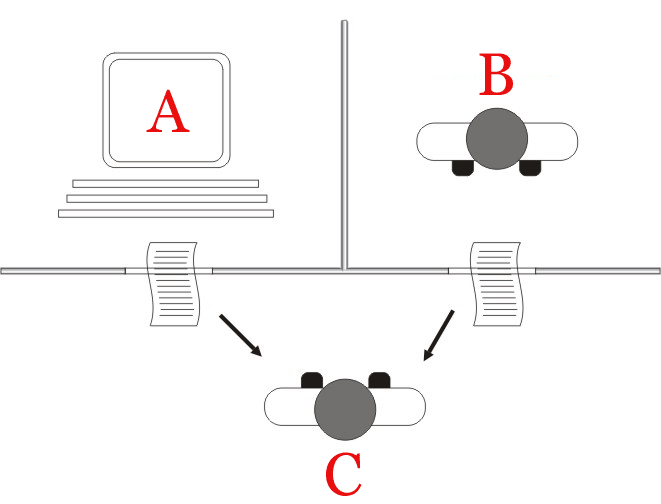
\includegraphics[width= 1\linewidth]{Turing_test}
		\caption{\small\textit{\color{cackithi}Hình $3$: Bài kiểm tra Turing.}}
		\vspace*{-10pt}
	\end{figure}
	Bài kiểm tra Turing được coi là đề xuất nghiêm túc đầu tiên trong triết lý trí tuệ nhân tạo. Dù bản thân sự mô tả khá đơn giản, việc chế tạo một cỗ máy có khả năng vượt qua bài kiểm tra lại có ý nghĩa sâu rộng. Cỗ máy đó sẽ phải xử lý ngôn ngữ tự nhiên, có thể học hỏi từ cuộc trò chuyện, ghi nhớ những gì đã được nói và truyền đạt ý tưởng trở lại con người, hiểu các khái niệm chung và hiển thị những gì chúng ta gọi là lẽ thường. 
	\vskip 0.1cm
	Ý tưởng về một vấn đề khó khăn, lâu dài như vậy là chìa khóa để định hình lĩnh vực AI vì nó đi thẳng vào trọng tâm của vấn đề -- thay vì giải quyết một vấn đề nhỏ, nó xác định mục tiêu cuối cùng có thể kéo nghiên cứu theo nhiều con đường. Nếu không có tầm nhìn về những gì AI có thể đạt được, bản thân lĩnh vực này có thể sẽ không bao giờ hình thành hoặc đơn giản vẫn chỉ là một nhánh của toán học hay triết học. 
	\vskip 0.1cm
	\textbf{\color{cackithi}Sự ra đời của AI}
	\vskip 0.1cm
	Năm $1952$, nhà khoa học máy tính Arthur Samuel tại IBM đã viết chương trình học chơi cờ đam trên máy tính IBM $701$, đánh dấu sự ra đời của lĩnh vực học máy. Máy tính IBM càng chơi càng tiến bộ, có thể nghiên cứu những nước đi nào tạo nên chiến lược chiến thắng và kết hợp những nước đi đó vào chương trình của mình. Sự thành công này đã bác bỏ quan niệm trước đây rằng máy tính không thể “học” mà chỉ làm được những điều được lập trình sẵn.
	\begin{figure}[H]
		\vspace*{-5pt}
		\centering
		\captionsetup{labelformat= empty, justification=centering}
		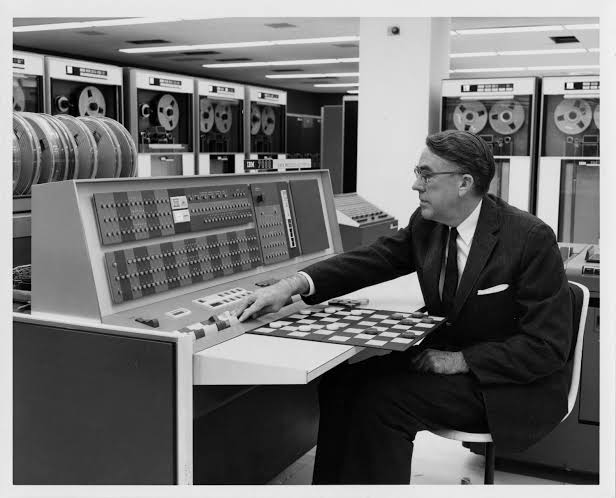
\includegraphics[width= 1\linewidth]{Samuel_Checker.jpeg}
		\caption{\small\textit{\color{cackithi}Hình $4$: Samuel chơi cờ với máy tính trên truyền hình. Nguồn: IBM.}}
		\vspace*{-10pt}
	\end{figure}
	Năm $1955$, hai nhà khoa học Allen Newell và Herbert Simon tại Đại học Carnegie Mellon cùng lập trình viên Cliff Shaw tại Tập đoàn Nghiên cứu và Phát triển (RAND) đã cho ra đời \textit{Logic Theorist}, một chương trình được thiết kế để mô phỏng kỹ năng giải quyết vấn đề của các nhà toán học. Chương trình khám phá cây tìm kiếm với gốc là giả thuyết ban đầu, mỗi nhánh là một suy luận dựa trên các quy tắc logic. Đâu đó trên cây là mệnh đề mà chương trình dự định chứng minh. Con đường dọc theo các nhánh dẫn từ giả thuyết đến mệnh đề cần phải chứng minh là một chứng minh. Logic Theorist đã chứng minh được $38$ trong số $52$ định lý đầu tiên trong chương hai bộ sách nổi tiếng \textit{Principia Mathematica} của Whitehead và Russell, trong đó có những chứng minh mới và ngắn hơn. Logic Theorist đã giới thiệu \textit{Lý luận thông qua tìm kiếm} và \textit{Phương pháp suy nghiệm} (Heuristic)\footnote{\color{cackithi}Phương pháp giải quyết vấn đề hoặc tự khám phá bằng cách sử dụng những biện pháp nhanh chóng để tạo ra các giải pháp đủ tốt trong một khoảng thời gian giới hạn.}, những khái niệm trọng tâm trong nghiên cứu AI sau này.
	\vskip 0.1cm
	Mùa hè năm $1956$, hội thảo về trí tuệ nhân tạo đầu tiên do Marvin Minsky, Nathaniel Rochester, Claude Shannon và John McCarthy tổ chức đã diễn ra ở Đại học Dartmouth. Trong số những người tham dự có Arthur Samuel, Herbert A. Simon và Allen Newell. Dưới sự thuyết phục của McCarthy, ``Trí tuệ nhân tạo" (Artificial Intelligence) đã được mọi người công nhận để chỉ lĩnh vực nghiên cứu mới, được Minsky định nghĩa như \textit{``lĩnh vực khoa học chế tạo máy móc làm được những việc đòi hỏi trí thông minh của con người"}. Hội thảo Dartmouth đã đánh dấu sự ra đời của trí tuệ nhân tạo như một lĩnh vực học thuật. Mặc dù không thu được những kết quả như kỳ vọng nhưng hội thảo đã là chất xúc tác cho hai mươi năm nghiên cứu AI sau đó.
	\begin{figure}[H]
		\vspace*{-5pt}
		\centering
		\captionsetup{labelformat= empty, justification=centering}
		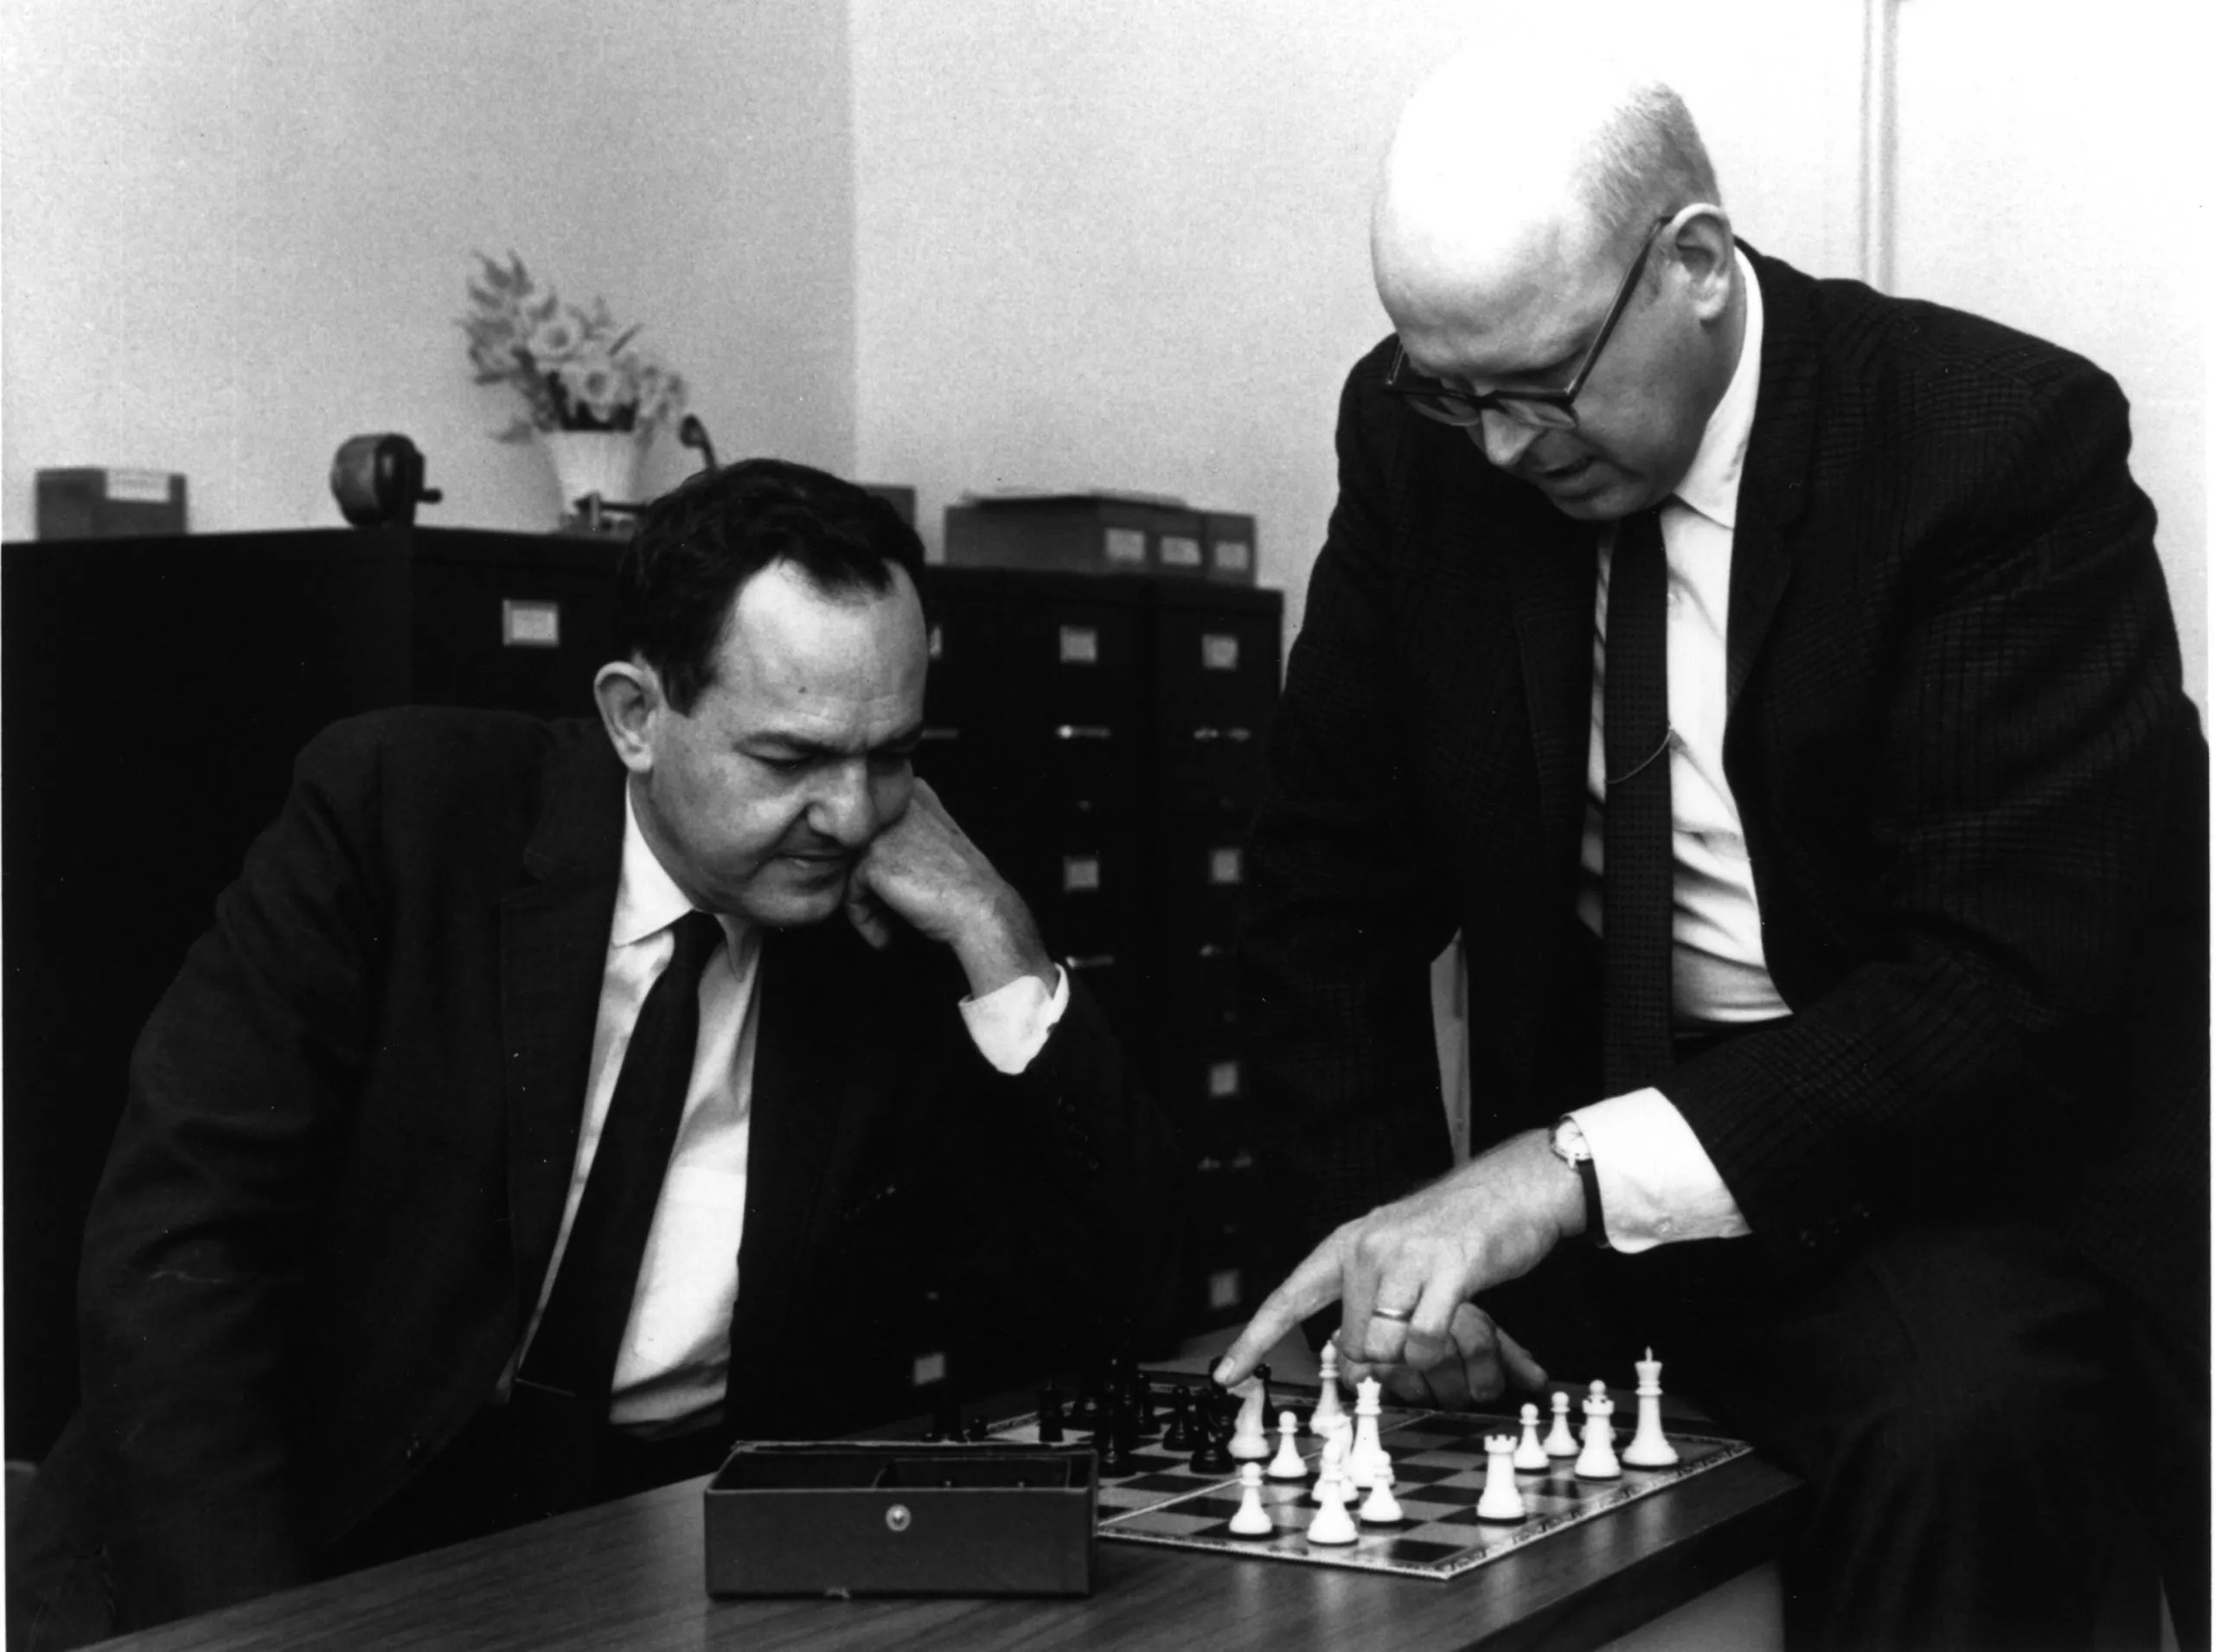
\includegraphics[width= 1\linewidth]{Newell_Simon.jpeg}
		\caption{\small\textit{\color{cackithi}Hình $5$: Herbert Simon (trái) và Allen Newell (phải). Nguồn: Đại học Carnegie Mellon.}}
		\vspace*{-10pt}
	\end{figure}
	\textbf{\color{cackithi}Đợt bùng nổ đầu tiên}
	\vskip 0.1cm
	Từ năm $1957$ đến năm $1974$, lĩnh vực AI phát triển mạnh mẽ. Sự ra đời của bóng bán dẫn thay thế đèn chân không giúp máy tính lưu trữ nhiều thông tin hơn, trở nên nhanh hơn, rẻ hơn và dễ tiếp cận hơn. Các thuật toán học máy cũng được cải thiện và mọi người hiểu rõ hơn rằng thuật toán nào sẽ áp dụng cho vấn đề của họ.
	\begin{figure}[H]
		\vspace*{5pt}
		\centering
		\captionsetup{labelformat= empty, justification=centering}
		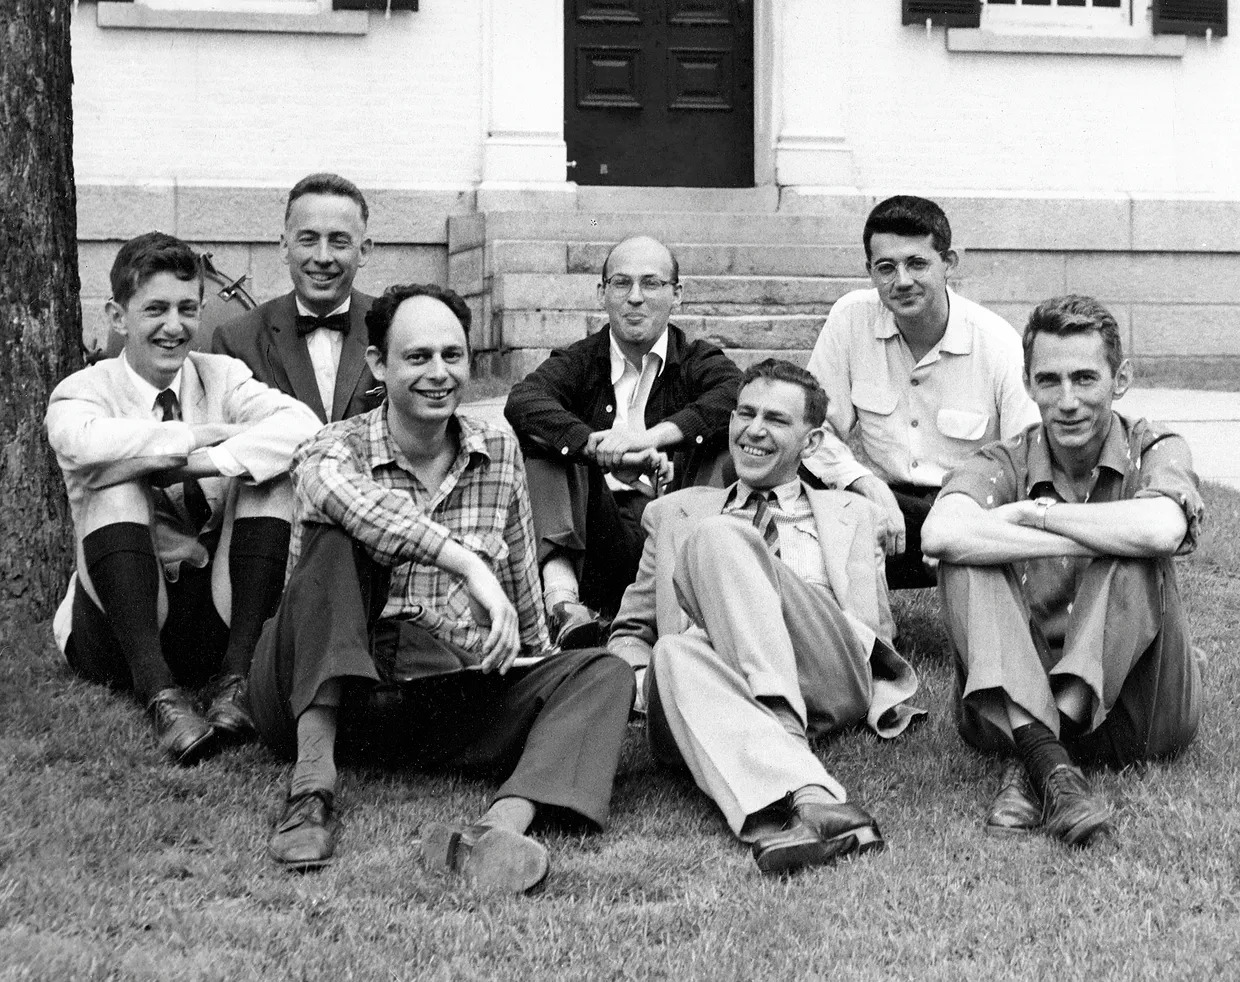
\includegraphics[width= 1\linewidth]{Dartmouth.jpg}
		\caption{\small\textit{\color{cackithi}Hình $6$: Hội thảo Dartmouth năm $1956$.\\ Nguồn: IEEE Spectrum.}}
		\vspace*{-10pt}
	\end{figure}
	Năm $1957$, Herbert Simon, Cliff Shaw và Allen Newell phát triển \textit{General Problem Solver}, hay GPS, một chương trình có mục địch giải quyết các vấn đề chung. GPS có thể giải được nhiều câu đố ấn tượng trong logic, hình học, đố chữ hay cờ vua thông qua phương pháp thử và sai (trial and error). GPS (cùng với Logic Theorist) đặt nền móng cho \textit{AI biểu tượng} (Symbolic AI), một nhánh của AI xem việc biểu diễn tri thức và lý luận dựa trên các quy tắc logic như là chìa khóa của trí thông minh. Với những đóng góp to lớn này, Newell và Simon được trao Giải thưởng Turing năm $1975$, giải thưởng danh giá được xem như Nobel của khoa học máy tính.\footnote{\color{cackithi}Herbert Simon cũng được trao Nobel kinh tế năm $1978$ cho những nghiên cứu tiên phong về quá trình ra quyết định trong các tổ chức kinh tế.}
	\begin{figure}[H]
		\vspace*{-5pt}
		\centering
		\captionsetup{labelformat= empty, justification=centering}
		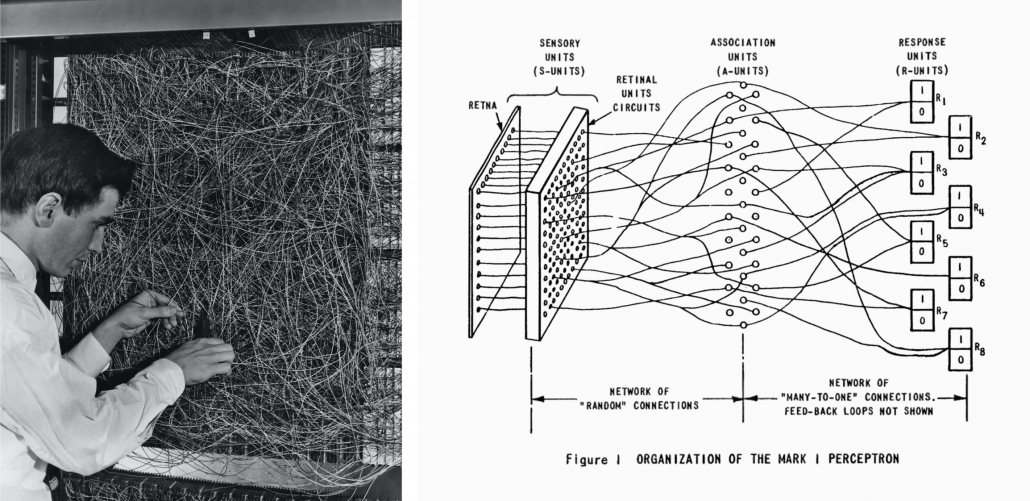
\includegraphics[width= 1\linewidth]{perceptron_1.png}
		\caption{\small\textit{\color{cackithi}Hình $7$: Frank Rosenblatt và Perceptron.\\ Nguồn: Researchgate.}}
		\vspace*{-10pt}
	\end{figure}
	Cùng năm $1957$, Frank Rosenblatt tại Phòng thí nghiệm Hàng không Cornell đã xây dựng \textit{Perceptron}, mạng thần kinh nhân tạo (một lớp) đầu tiên lấy cảm hứng từ mô hình toán học của não bộ phát triển bởi Warren S. McCulloch và Walter Pitts những năm $1940$. Perceptron được viết trên IBM $704$, một máy tính $5$ tấn có kích thước của một căn phòng. Sau $50$ lần thử, máy tự học cách phân biệt các thẻ được đánh dấu bên trái với các thẻ được đánh dấu bên phải. Perceptron đánh dấu sự ra đời của chủ nghĩa kết nối, nền tảng của \textit{Mạng thần kinh}  và \textit{Học sâu} được phát triển sau này.
	\vskip 0.1cm
	Năm $1960$, John McCarthy \footnote{\color{cackithi}Giải thưởng Turing $1971$.} tại Viện Công nghệ Massachusetts (MIT) đã phát triển \textit{LISP}, một ngôn ngữ lập trình bậc cao dựa trên giải tích lambda. LISP trở nên rất quan trọng cho sự phát triển ban đầu của AI nhờ khả năng xử lý biểu tượng và tính linh hoạt trong việc quản lý các tác vụ phức tạp. Tuy vậy, phải đến đầu những năm $1970$, với sự ra đời của máy tính mạnh mẽ hơn sử dụng mạch tích hợp (chip silicon chứa nhiều bóng bán dẫn), các lập trình viên mới có thể triển khai các ứng dụng tri thức sâu rộng.
	\begin{figure}[H]
		\vspace*{-5pt}
		\centering
		\captionsetup{labelformat= empty, justification=centering}
		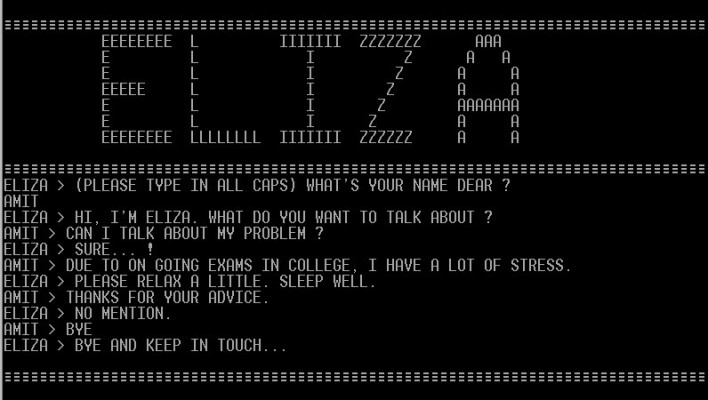
\includegraphics[width= 1\linewidth]{eliza.jpeg}
		\caption{\small\textit{\color{cackithi}Hình $8$: Tương tác với ELIZA.}}
		\vspace*{-10pt}
	\end{figure}
	Năm $1965$, Joseph Weizenbaum -- nhà khoa học máy tính và giáo sư tại MIT -- đã phát triển \textit{ELIZA}, một hệ thống xử lý ngôn ngữ tự nhiên mô phỏng bác sĩ. ELIZA trả lời các câu hỏi trong bối cảnh một buổi trị liệu tâm lý. ELIZA xác định các từ khóa từ dữ liệu đầu vào của người dùng và khớp chúng với các câu trả lời được lập trình sẵn. Một số người dùng tin rằng họ đang tương tác với một người khác cho đến khi chương trình đạt đến giới hạn và cuộc trò chuyện trở nên vô nghĩa. ELIZA là tiền thân của những chatbot ngày nay.
	\vskip 0.1cm
	Bị thu hút bởi những kỳ vọng cùng sự lạc quan của các nhà khoa học hàng đầu, chính phủ Mỹ đã tài trợ ồ ạt cho nghiên cứu AI. Chính phủ đặc biệt quan tâm đến một cỗ máy có thể phiên âm và dịch ngôn ngữ nói cũng như xỷ lý dữ liệu thông lượng cao. Cơ quan Nghiên cứu Quốc phòng Tiên tiến (DARPA) đã đầu tư hàng triệu USD để hỗ trợ nghiên cứu AI tại một số cơ sở nghiên cứu như MIT, Đại học Stanford, Đại học Carnegie Mellon cũng như một số phòng thí nghiệm nghiên cứu thương mại khác. Năm $1970$, Marvin Minsky (giáo sư tại MIT, giải thưởng Turing $1969$) nói với Tạp chí Life: \textit{``Từ ba đến tám năm nữa chúng ta sẽ có một cỗ máy có trí thông minh chung của một con người bình thường"}. 
	\vskip 0.1cm
	\textbf{\color{cackithi}Mùa đông AI\footnote{\color{cackithi}Được mượn từ cụm từ ``Mùa đông hạt nhân", một lý thuyết thời Chiến tranh Lạnh cho rằng việc sử dụng vũ khí hạt nhân hàng loạt sẽ che khuất Mặt Trời bằng khói và bụi, khiến nhiệt độ toàn cầu giảm mạnh, Trái Đất đóng băng và nhân loại tuyệt chủng.}}
	\vskip 0.1cm
	Những kỳ vọng cao và những tuyên bố đầy tham vọng thường là con đường trực tiếp dẫn đến sự thất vọng. Các nhà nghiên cứu AI đã quá lạc quan trong việc thiết lập các mục tiêu của họ và đã đưa ra những giả định ngây thơ về những khó khăn mà họ sẽ gặp phải. Việc phá vỡ lớp sương mù ban đầu của AI đã bộc lộ một núi chướng ngại vật. 
	\vskip 0.1cm
	Trước hết, AI gặp phải những rào cản công nghệ không thể vượt qua, chủ yếu là hạn chế về sức mạnh tính toán, bộ nhớ và tốc độ xử lý. Vào giữa những năm $1960$, các nhà nghiên cứu đã phát hiện ra sự khác biệt giữa sự tăng trưởng đa thức và tăng trưởng cấp số nhân trong độ phức tạp của bài toán. Độ phức tạp tăng trưởng theo cấp số nhân ngăn cản việc giải quyết các vấn đề cỡ lớn vừa phải trong một khoảng thời gian hợp lý. Điều này dẫn đến khái niệm quan trọng nhất trong lý thuyết độ phức tạp, \textit{tính  $NP$--đầy đủ} ($NP$--completeness) và câu hỏi cơ bản nhất của nó, liệu $P = NP$, trong đó $P$ là lớp các câu hỏi mà tồn tại thuật toán có thể \textit{giải} trong thời gian đa thức và $NP$ là lớp các câu hỏi mà câu trả lời (cho trước) có thể được \textit{xác minh} trong thời gian đa thức.\footnote{\color{cackithi}Một trong bảy bài toán thiên niên kỷ của viện toán Clay.} Nhiều bài toán tổ hợp và logic là $NP$--đầy đủ, đòi hỏi thời gian giải theo cấp số nhân và các hệ thống không có khả năng giải quyết một cách hiệu quả.
	\vskip 0.1cm
	Thêm vào đó, các nhà nghiên cứu đã tập trung nhiều vào khía cạnh lý thuyết và đánh giá thấp sự phức tạp đến từ các vấn đề thực tiễn. Sau khi giải mã thành công mật mã của Đức trong Thế chiến thứ hai, các nhà khoa học đã lầm tưởng rằng việc dịch văn bản giữa các ngôn ngữ sẽ không khó hơn việc giải mã mật mã. Trên thực tế, việc xử lý ngôn ngữ tự nhiên trong dịch máy đòi hỏi những hiểu biết sâu sắc về ngôn ngữ học. Người ta cần biết nghĩa của nhiều từ và hiểu chúng theo nhiều cách kết hợp. Nỗ lực tự động tra cứu từ điển và áp dụng các quy tắc ngữ pháp đã không đem lại kết quả. 
	\vskip 0.1cm
	Năm $1969$, trong cuốn sách \textit{Perceptrons}, Marvin Minsky và Seymour Papert đã công kích công trình Perceptron của Rosenblatt và chỉ những hạn chế của mạng thần kinh nhân tạo. Cuốn sách có ảnh hưởng lớn và được xem là nguyên nhân chính dẫn đến sự đình trệ trong việc nghiên cứu mạng thần kinh những năm $1970$.
	\vskip 0.1cm
	Sau hai thập kỷ với hàng chục triệu đô la đầu tư mà không nhận được những giải pháp như kỳ vọng, cộng với những khó khăn về tài chính, chính phủ Mỹ và Anh lần lượt cắt giảm các nguồn tài trợ cho AI, dẫn đến sự sụt giảm đáng kể các hoạt động AI trong cả công nghiệp và các viện nghiên cứu. Mùa đông AI đầu tiên kéo dài từ $1974$ đến $1980$.
	\vskip 0.1cm
	\textbf{\color{cackithi}Hệ thống chuyên gia}
	\vskip 0.1cm
	Vào những năm $1970$, nghiên cứu AI tập trung vào AI biểu tượng với trọng tâm là các lĩnh vực chuyên môn được đánh giá cao và phức tạp. Với ý tưởng \textit{``các hệ thống thông minh có được sức mạnh từ kiến thức mà chúng sở hữu chứ không phải từ các hình thức và sơ đồ suy luận cụ thể mà chúng sử dụng"}, Edward Feigenbaum \footnote{\color{cackithi}Giải thưởng Turing $1994$.} tại Đại học Stanford cùng các đồng nghiệp đã phát triển các hệ thống chuyên gia -- hay hệ thống dựa trên tri thức -- chương trình máy tính mô phỏng quá trình ra quyết định của các chuyên gia. 
	\begin{figure}[H]
		\vspace*{-5pt}
		\centering
		\captionsetup{labelformat= empty, justification=centering}
		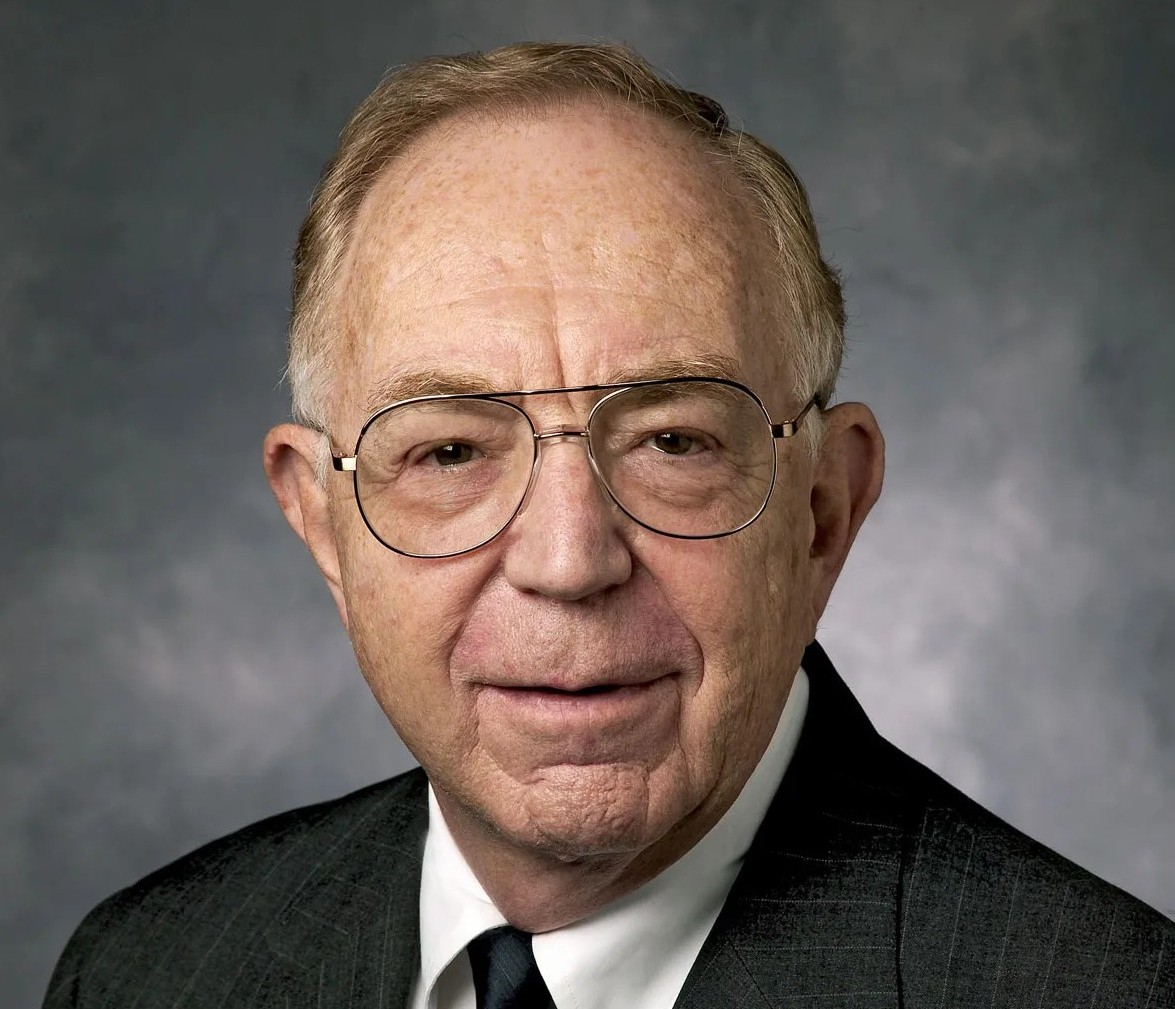
\includegraphics[width= 1\linewidth]{Edward-Feigenbaum.jpeg}
		\caption{\small\textit{\color{cackithi}Hình $9$: Edward Feigenbaum. Nguồn: Britannica.}}
		\vspace*{-10pt}
	\end{figure}
	Một hệ thống chuyên gia bao gồm hai thành phần cơ bản: cơ sở tri thức và công cụ suy luận. Cơ sở tri thức lưu trữ thông tin, được thu thập bằng cách phỏng vấn những người là chuyên gia trong lĩnh vực được đề cập và được sắp xếp thành một tập hợp các quy tắc, thường có cấu trúc ``NẾU--THÌ" (if--then). Chẳng hạn: ``NẾU bệnh nhân bị sốt VÀ bệnh nhân ho VÀ bệnh nhân khó thở THÌ bệnh nhân có thể bị viêm phổi". Công cụ suy luận cho phép hệ thống chuyên gia rút ra các suy luận từ các quy tắc trong cơ sở tri thức. Ví dụ: nếu cơ sở tri thức chứa quy tắc ``NẾU $x$ THÌ $y$" và ``NẾU $y$ THÌ $z$", công cụ suy luận có thể suy ra ``NẾU $x$ THÌ $z$". Sau đó, hệ thống chuyên gia có thể truy vấn người dùng (có thể không phải chuyên gia) ``$x$ có đúng trong tình huống mà chúng ta đang xem xét không?" Nếu câu trả lời là khẳng định, hệ thống sẽ tiến hành suy ra $z$.
	\begin{figure}[H]
		\vspace*{-5pt}
		\centering
		\captionsetup{labelformat= empty, justification=centering}
		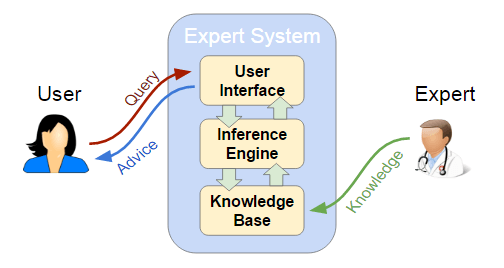
\includegraphics[width= 0.9\linewidth]{Expert_System.png}
		\caption{\small\textit{\color{cackithi}Hình $10$: Hệ thống chuyên gia.}}
		\vspace*{-10pt}
	\end{figure}
	Sau thành công của hệ thống DENDRAL trong việc xác định các phân tử hữu cơ chưa biết và MYCIN trong việc chẩn đoán các bệnh truyền nhiễm vào thập niên $1970$, hệ thống chuyên gia thương mại được sử dụng rộng rãi trong chẩn đoán y tế, phân tích hóa học, tín dụng ủy quyền, quản lý tài chính, thăm dò dầu và khoáng sản, kỹ thuật di truyền, thiết kế và sản xuất ô tô, thiết kế lắp đặt máy tính, lập kế hoạch hàng không, sắp xếp hàng hóa và các dịch vụ, v.v. Các hệ thống chuyên gia cho thấy những lợi thế khác biệt so với các chương trình máy tính truyền thống. Chúng có thể  cung cấp các lựa chọn và các vấn đề cho người ra quyết định cũng như hỗ trợ việc ra quyết định trong trường hợp quyết định đó vượt quá trình độ kiến thức và kinh nghiệm của họ. Ngược lại với con người, hệ thống chuyên gia có thể  lưu trữ vĩnh viễn kiến thức chuyên môn, đưa ra mức độ tham vấn nhất quán sau khi được lập trình. Với kiến thức có được từ nhiều chuyên gia, các hệ thống này có thể cung cấp, hỗ trợ việc ra quyết định một cách toàn diện. Theo khảo sát những năm $1980$, khoảng $2/3$ trong số $500$ tập đoàn lớn nhất của Mỹ lúc bấy giờ sử dụng hệ thống chuyên gia trong hoạt động kinh doanh thường nhật.
	\vskip 0.1cm
	Đứng trước những triển vọng to lớn, chính phủ nhiều nước đã đầu tư mạnh mẽ cho nghiên cứu và phát triển các hệ thống AI. Năm $1981$, Bộ Kinh tế, Thương mại và Công nghiệp Nhật Bản phân bổ ngân sách $850$ triệu USD cho dự án máy tính thế hệ thứ năm với tham vọng dẫn đầu thế giới về công nghệ máy tính. Mục tiêu của Nhật Bản là tạo ra những cỗ máy có thể nói chuyện với con người, dịch ngôn ngữ, diễn giải hình ảnh và suy luận như con người. Đáp lại, các chính phủ Mỹ, Anh và Châu Âu cũng đẩy mạnh tài trợ cho nghiên cứu AI. Đến năm $1985$, khoản đầu tư của Mỹ vào hệ thống chuyên gia AI đã đạt hơn $1$ tỷ USD. Vương quốc Anh cũng bắt đầu dự án Alvey trị giá $350$ triệu bảng Anh.
	\vskip 0.1cm
	Một lần nữa, kỳ vọng đã cao hơn nhiều so với mức thực tế có thể thực hiện được. Đến cuối những năm $1980$, các hệ thống chuyên gia dần bộc lộ nhiều vấn đề và hạn chế về công nghệ khó giải quyết. Trước tiên, việc thu thập dữ liệu và thiết kế các quy tắc đòi hỏi rất nhiều công sức. Trên thực tế, các chuyên gia chỉ có thể diễn đạt bằng lời một phần nhỏ kiến thức của họ. Thêm vào đó, những hệ thống nhiều hơn $200$ quy tắc có thể xuất hiện hiệu ứng ``hộp đen" -- chúng ta không rõ máy suy luận như thế nào.\footnote{\color{cackithi}Những hệ thống chuyên gia lớn thường có trên $1000$ quy tắc.} Các hệ thống chuyên gia cũng tỏ ra rất tốn kém để bảo trì. Chúng khó cập nhập, không có khả năng học và có thể mắc những sai lầm ngớ ngẩn khi được cung cấp thông tin đầu vào bất thường. 
	\vskip 0.1cm
	Từ cuối những năm $1980$, chính phủ Mỹ và Nhật Bản lần lượt chấm dứt các nguồn tài trợ cho AI để tập trung vào các dự án nhanh đem lại kết quả. Như một hệ quả, AI trải qua mùa đông thứ hai, kéo dài đến năm $2000$.
	\vskip 0.1cm
	\textbf{\color{cackithi}Học máy và học sâu}
	\vskip 0.1cm
	Năm $1997$, đương kim vô địch cờ vua thế giới Gary Kasparov đã bị đánh bại bởi Deep Blue, một hệ thống chuyên gia chơi cờ vua của IBM. Trận đấu được công bố rộng rãi và trở thành biểu tượng trong lịch sử. Tuy vậy, thành công này không còn hỗ trợ cho sự phát triển của AI biểu tượng. Trên thực tế, Deep Blue và những hệ thống chuyên gia khác chỉ xử lý được một phạm vi rất hạn chế (như là là quy tắc của ván cờ), rất xa so sự phức tạp của thế giới thực.
	\begin{figure}[H]
		\vspace*{-5pt}
		\centering
		\captionsetup{labelformat= empty, justification=centering}
		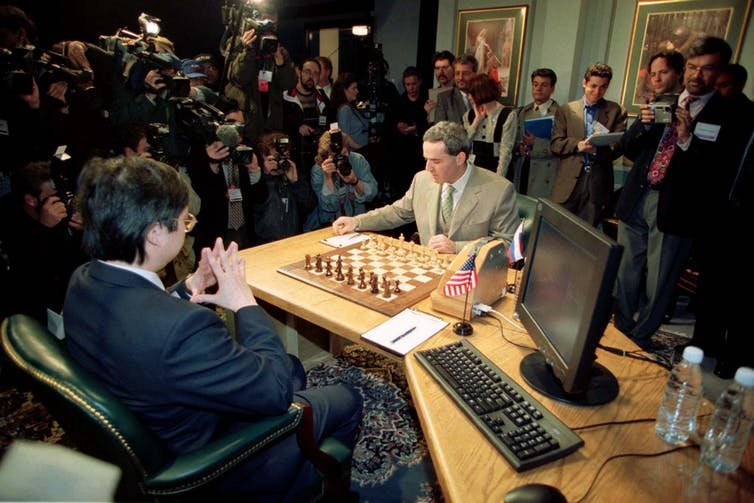
\includegraphics[width= 1\linewidth]{DeepBlue.jpg}
		\caption{\small\textit{\color{cackithi}Hình $11$: Kasparov đối đầu Deep Blue. Nguồn: Sportshistoryweekly.}}
		\vspace*{-10pt}
	\end{figure}
	Từ những năm $1990$, trọng tâm của nghiên cứu về AI đã chuyển từ cách tiếp cận dựa trên tri thức sang cách tiếp cận dựa trên dữ liệu (học máy). Thay vì mã hóa quy tắc cho các hệ thống AI như trước kia, các nhà khoa học tạo ra các chương trình máy tính để phân tích lượng lớn dữ liệu và rút ra kết luận -- hay ``học" -- từ kết quả (Hình $12$). Sự chuyển dịch này là kết quả của sự phát triển của Internet. Học máy được hưởng lợi từ sự sẵn có ngày càng tăng của dữ liệu số và khả năng chia sẻ các dịch vụ của mình qua Internet. 
	\vskip 0.1cm
	Nhằm giải quyết các vấn đề phức tạp cũng như cung cấp các giải pháp hữu ích trong các lĩnh vực ứng dụng khác nhau, các nhà nghiên cứu AI bắt đầu sử dụng và phát triển các công cụ toán học phức tạp hơn. Họ nhận ra rằng nhiều vấn đề về AI đã được các nhà nghiên cứu trong các lĩnh vực như toán học, kinh tế hoặc vận trù học giải quyết. Chẳng hạn, các mạng thần kinh nhân tạo không gì khác hơn là các mô hình hồi quy phi tuyến tính và mô hình khác biệt (Discriminant models) và có thể được phân tích bằng phần mềm thống kê tiêu chuẩn, giống như nhiều mô hình thống kê khác. Sử dụng ngôn ngữ toán học cho phép sự cộng tác ở mức độ cao hơn giữa các lĩnh vực khác nhau và khiến AI trở thành một ngành khoa học chặt chẽ hơn.
	\begin{figure}[H]
		\vspace*{-5pt}
		\centering
		\captionsetup{labelformat= empty, justification=centering}
		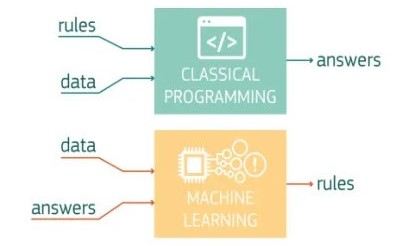
\includegraphics[width= 0.9\linewidth]{ML-TraditionalProgramming.jpeg}
		\caption{\small\textit{\color{cackithi}Hình $12$: Sự khác nhau giữa các chương trình truyền thống và học máy. Trong học máy, dữ liệu đầu vào (data) và đầu ra (answers) được đưa vào thuật toán để tạo ra chương trình (rules). Chương trình này có thể được sử dụng để dự đoán kết quả trong tương lai. Nguồn: [$3$].}}
		\vspace*{-10pt}
	\end{figure}
	Năm $2004$, Geoffrey Hinton (Đại học Toronto), Yoshua Bengio (Đại học Montreal) và Yann LeCun (Đại học New York) dưới sự tài trợ của chính phủ Canada đã bắt đầu một chương trình nghiên cứu để cập nhật mạng thần kinh nhân tạo. Các thí nghiệm được tiến hành đồng thời tại Microsoft, Google và IBM với sự trợ giúp của phòng thí nghiệm của Hinton  ở Toronto cho thấy kiểu học này đã thành công trong việc giảm một nửa tỷ lệ lỗi trong nhận dạng giọng nói. Nhóm nhận dạng hình ảnh của Hinton cũng đạt được kết quả tương tự. Thuật ngữ ``học sâu" được Geoffrey Hinton đặt cho các thuật toán mới này. Trong một thời gian ngắn, phần lớn các nhóm nghiên cứu đã chuyển sang sử dụng công nghệ này với những lợi ích không thể chối cãi.\footnote{\color{cackithi}Bengio, Hilton và LeCun được trao Giải thưởng Turing năm $2018$ cho việc cách mạng hóa lĩnh vực học sâu.} 
	\begin{figure}[H]
		\vspace*{5pt}
		\centering
		\captionsetup{labelformat= empty, justification=centering}
		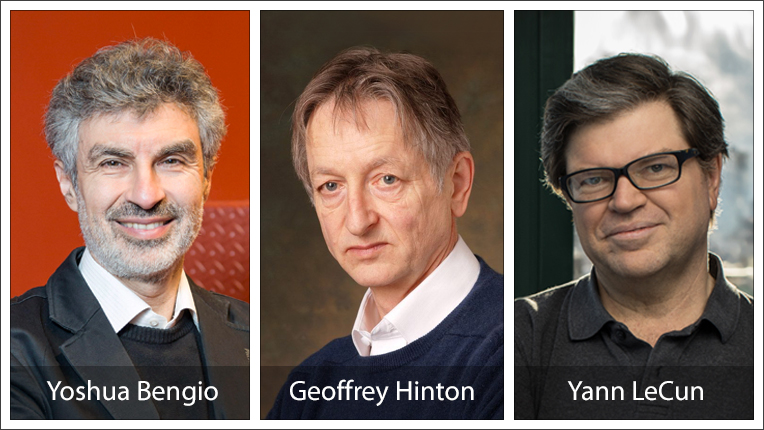
\includegraphics[width= 1\linewidth]{turing-2018-bengio-hinton-lecun.jpg}
		\caption{\small\textit{\color{cackithi}Hình $13$: Giải thưởng Turing $2018$. Nguồn: AMC.}}
		\vspace*{-15pt}
	\end{figure}
	Kể từ năm $2010$, lĩnh vực học sâu phát triển chóng mặt. 
	\vskip 0.1cm
	Năm $2011$, IBM Watson, một hệ thống máy tính có khả năng trả lời các câu hỏi được đặt ra bằng ngôn ngữ tự nhiên đã thắng trò chơi Jeopardy!\footnote{\color{cackithi}Chương trình đố vui ngược với hình thức hỏi đáp truyền thống trên truyền hình của Mỹ. Thí sinh được cung cấp những manh mối kiến thức chung dưới dạng câu trả lời và họ phải diễn đạt từng câu trả lời dưới dạng một câu hỏi.} trước Ken Jennings và Brad Rutter, hai trong số những thí sinh thành công nhất trong chương trình này, và giành được $1$ triệu USD. Máy tính của IBM áp dụng các công nghệ xử lý ngôn ngữ tự nhiên tiên tiến, truy xuất thông tin, biểu diễn tri thức, lý luận tự động và học máy vào lĩnh vực trả lời câu hỏi trong miền mở. Cùng năm, Apple cho ra mắt Siri, trợ lý ảo đầu tiên được sử dụng rộng rãi.
	\vskip 0.1cm
	Năm $2016$, AlphaGo, phát triển bởi DeepMind, đã đánh bại Lee Sedol, một trong số những kỳ thủ cờ vây xuất sắc nhất thế giới. Vì tính phức tạp của nó, cờ vây (Go) lúc đó được coi là nằm ngoài tầm với của AI trong ít nhất một thập kỷ nữa. AlphaGo sử dụng mạng thần kinh nhân tạo sâu, được đào tạo thông qua \textit{học tăng cường}. Một năm sau, AlphaGo được nâng cấp thành AlphaZero, chương trình mạnh mẽ hơn có thể chơi được cả cờ vua, cờ vây và cờ tướng Nhật Bản (Shogi).
	\vskip 0.1cm
	Vào tháng $11$ năm $2020$, mô hình AlphaFold của DeepMind, một hệ thống học sâu được thiết kế để xác định cấu trúc ba chiều của protein, đã mang lại kết quả cực kỳ chính xác, tạo ra một bước tiến vượt bậc trong cái mà các nhà khoa học gọi là ``vấn đề gấp protein". Vào tháng $7$ năm $2022$, DeepMind thông báo rằng AlphaFold có thể xác định cấu trúc của gần $200$ triệu protein từ $1$ triệu loài, bao gồm hầu hết mọi loại protein mà con người biết đến. Khả năng của AlphaFold đã mở ra cánh cửa cho các nhà nghiên cứu y tế phát triển rất nhiều các loại thuốc và vắc xin phục vụ nhân loại.
	\begin{figure}[H]
		\vspace*{-5pt}
		\centering
		\captionsetup{labelformat= empty, justification=centering}
		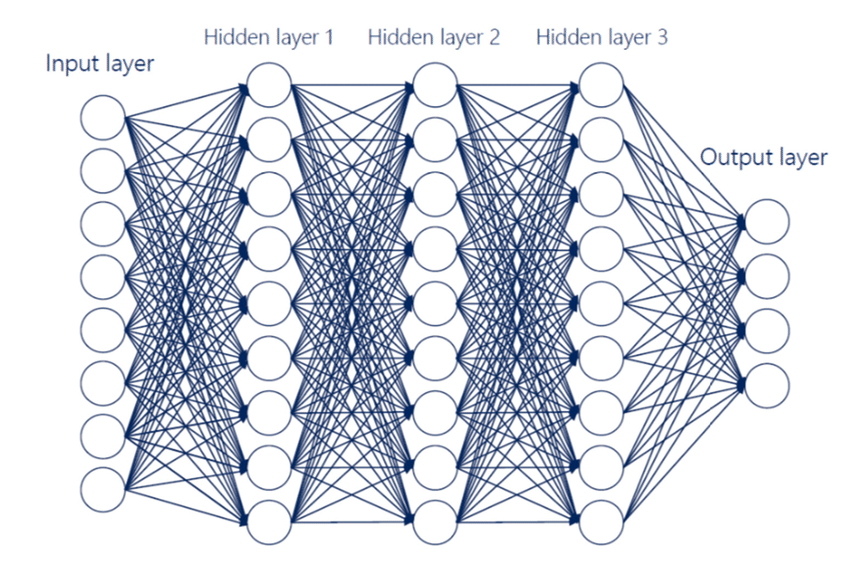
\includegraphics[width= 1\linewidth]{Deep-Neural-Network.png}
		\caption{\small\textit{\color{cackithi}Hình $14$: Một ví dụ về mạng thần kinh nhân tạo sâu đơn giản gồm lớp đầu vào, lớp đầu ra và $3$ lớp ẩn. Mỗi nơron trong một lớp được kết nối với tất cả các nơron ở lớp trước (và sau).}}
		\vspace*{-10pt}
	\end{figure}
	Những thành công và triển vọng to lớn được mở ra bởi lĩnh vực học máy, đặc biệt là học sâu đã thúc đẩy các tập đoàn công nghệ tư nhân như Google, Microsoft, Facebook, Tesla, Alibaba v.v. đầu tư mạnh mẽ vào AI, được theo sau bởi các chính phủ. Năm $2022$, tổng vốn đầu tư tư nhân cho AI toàn cầu đạt $92$ tỷ USD, trong đó Mỹ dẫn đầu với $47{,}4$ tỷ USD, theo sau là Trung Quốc với $13{,}4$ tỷ USD. Năm $2018$, chính phủ Trung Quốc đưa ra quy trình gồm ba giai đoạn đầy tham vọng với mục tiêu đưa Trung Quốc trở thành trung tâm AI ``chính" của thế giới vào năm $2030$. Cùng năm, Ủy ban châu Âu dự định phân bổ $1$ tỷ euro để đầu tư cho AI mỗi năm. Con số này dự định sẽ tăng lên $20$ tỷ euro mỗi năm vào thập kỷ tới. Các quốc gia Ấn Độ, Hàn Quốc, Canada, Nhật Bản, Israel, Nga và Singapore cũng đầu tư mạnh mẽ cho AI.
	\vskip 0.1cm
	\textbf{\color{cackithi}Định luật Moore}
	\vskip 0.1cm
	Những tiến bộ mà AI đạt được có sự đóng góp to lớn của những tiến bộ trong công nghệ máy tính. 
	\vskip 0.1cm
	Năm $1965$, Gordon E. Moore -- một trong những người tiên phong về mạch tích hợp, nhà đồng sáng lập và giám đốc điều hành của Intel sau này -- đưa ra dự đoán rằng số lượng bóng bán dẫn có thể được tích hợp trên một đơn vị không gian của mạch tích hợp sẽ tăng gấp đôi mỗi năm. Năm $1975$, ông sửa lại ước tính của mình thành tăng gấp đôi sau mỗi hai năm. Dự đoán này được gọi là \textit{Định luật Moore}. Các phép đo quan trọng khác cũng cho thấy hành vi nhân đôi tương tự, chẳng hạn như tốc độ bộ xử lý và dung lượng bộ nhớ phù hợp với máy tính. 
	\begin{figure}[H]
		\vspace*{-5pt}
		\centering
		\captionsetup{labelformat= empty, justification=centering}
		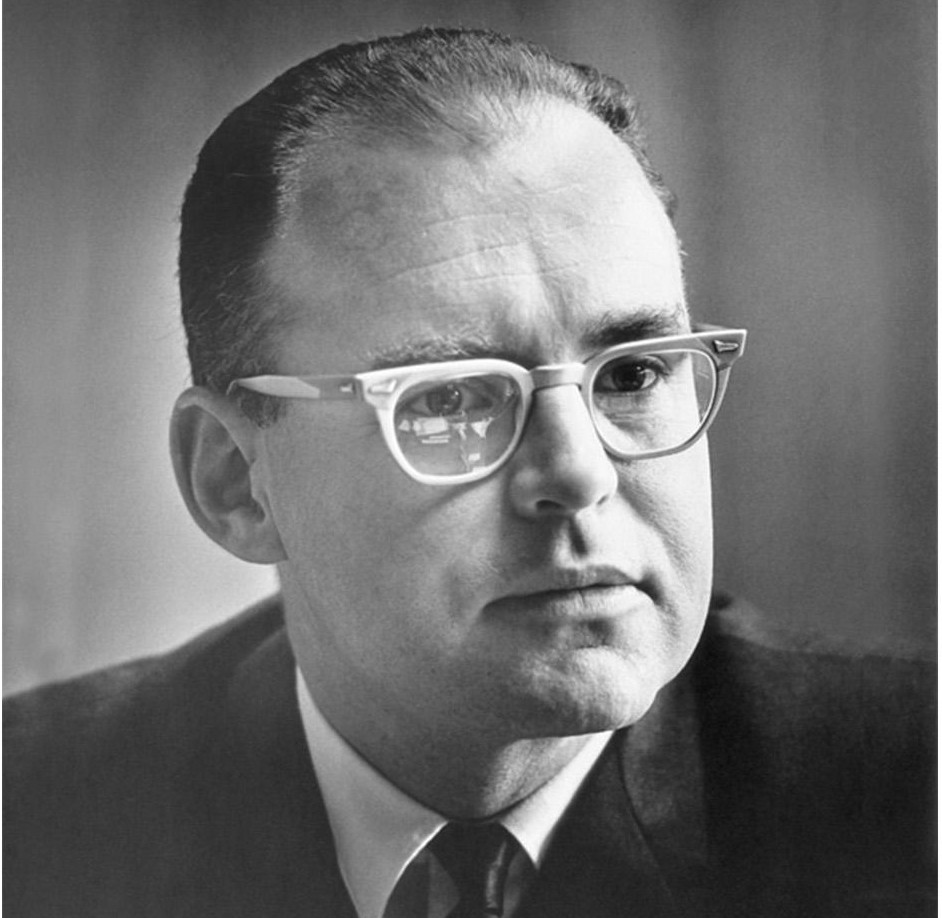
\includegraphics[width= 1\linewidth]{Gordon_E._Moore.jpg}
		\caption{\small\textit{\color{cackithi}Hình $15$: Gordon E. Moore. Nguồn: Intel.}}
		\vspace*{-10pt}
	\end{figure}
	Trong suốt sáu thập kỷ qua, định luật Moore được sử dụng như kim chỉ nam trong ngành công nghiệp bán dẫn. Tầm quan trọng của định luật này không chỉ ở việc dung lượng bộ nhớ ngày càng lớn và tốc độ máy tính ngày càng nhanh theo thời gian mà các kỹ sư có thể dự đoán quy mô lớn hơn và nhanh hơn bao nhiêu. Điều này giúp họ lập kế hoạch dài hạn cho các dự án phát triển phần mềm và phần cứng. 
	\vskip 0.1cm
	Định luật Moore có tác động lâu dài đến sự phát triển của AI. Việc tăng gấp đôi tốc độ phần cứng  hoặc gấp đôi bộ nhớ sẽ cải thiện quy mô của vấn đề mà ta có thể xử lý hiệu quả. Cách Deep Blue được mã hóa không khác nhiều so với các chương trình chơi cờ vua $30$ năm trước đó. Điều khác biệt ở đây là Deep Blue có khả năng tìm kiếm $200$ triệu thế cờ mỗi giây kế hợp với thông tin trong kho dữ liệu khổng lồ để chọn nước đi. Nó đưa ra một chút lời giải thích cho quá trình nghiên cứu AI: các nhà khoa học tạo ra các chương trình vượt quá sức mạnh tính toán hiện tại, sau đó chờ định luật Moore bắt kịp.
	\begin{figure}[H]
		\vspace*{-5pt}
		\centering
		\captionsetup{labelformat= empty, justification=centering}
		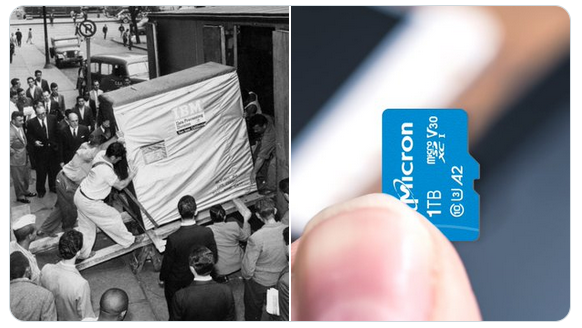
\includegraphics[width= 1\linewidth]{Disk.png}
		\caption{\small\textit{\color{cackithi}Hình $16$: Ổ cứng dung lượng $5$ MB năm $1956$ có giá trên $50{.}000$ USD so với thẻ nhớ $1$ TB ($1000{.}000$ MB) năm $2020$ có giá $100$ USD.}}
		\vspace*{-10pt}
	\end{figure}
	Từ năm $2010$, đã có những dấu hiệu cho thấy định luật Moore đang chậm lại. Tuy vậy, sự gia tăng dữ liệu cũng như sức mạnh tính toán mới đã đem đến động lực mới to lớn, dẫn đến sự bùng nổ của học sâu. Các nhà khoa học phát hiện ra hiệu quả rất cao của bộ xử lý đồ họa máy tính (GPU) trong việc đẩy nhanh quá trình tính toán các thuật toán học máy. Từ năm $2010$, tốc độ tính toán tăng theo cấp số nhân trước kia thậm chí còn nhanh hơn nữa, đạt gấp đôi chỉ trong vòng $6$ tháng. PaLM, một mô hình ngôn ngữ tự nhiên của Google, lớn hơn $5$ triệu lần so với AlexNet, hệ thống AI có tính toán đào tạo lớn nhất $10$ năm trước. Những đột phá trong công nghệ lượng tử, khoa học máy tính, toán học, vật lý hay học máy đều đóng vai trò là những bước đột phá tiềm năng vượt qua giới hạn của định luật Moore.
	\vskip 0.1cm
	\textbf{\color{cackithi}Tương lai}
	\vskip 0.1cm
	Bây giờ chúng ta quay trở lại hiện tại. Rất nhiều các ứng dụng thông minh đã hiện hữu trong cuộc sống hàng ngày, nhiều công nghệ mới chỉ gần đây còn là khoa học viễn tưởng giờ đã trở thành hiện thực. Vậy điều gì đang chờ đợi chúng ta phía trước?
	\vskip 0.1cm
	Theo Rodney Brooks, giáo sư Robotics tại MIT, thì việc dự đoán tương lai của AI là rất khó khăn. Ông dẫn ra luật Amara nổi tiếng:
	\textit{``Chúng ta có xu hướng đánh giá quá cao tác động của một công nghệ trong thời gian ngắn và đánh giá thấp tác động về lâu dài."}
	Luật Amara trình bày một mô hình được tìm thấy trong nhiều công nghệ mới nổi. Một lời hứa lớn trước mắt, sự thất vọng, và rồi sự tự tin dần dần tăng lên vượt xa những gì mong đợi ban đầu hướng tới. Nhiều công nghệ được đánh giá quá cao trong ngắn hạn, trong khi lợi ích lại được tích lũy về lâu dài. 
	\vskip 0.1cm
	Trước mắt, các \textit{mô hình ngôn ngữ lớn} (Large Language Models) và \textit{AI tạo sinh} (Generative AI) đang tạo ra những bước đột phá lớn tiếp theo. Người ta có thể tưởng tượng việc tương tác với một hệ thống chuyên gia trong một cuộc trò chuyện trôi chảy hoặc có một cuộc trò chuyện bằng hai ngôn ngữ khác nhau được dịch theo thời gian thực. Chúng ta cũng có thể kỳ vọng sẽ thấy những chiếc ô tô không người lái trên đường trong nhiều năm tới.
	\vskip 0.1cm
	Cũng giống nhiều mô hình trí tuệ nhân tạo khác, học sâu còn nhiều vấn đề cần được giải quyết, bao gồm các cuộc tấn công đối nghịch, tạo ra nội dung giả (deepfake), sự công bằng, trách nhiệm giải trình, tính minh bạch và các cân nhắc về đạo đức khác.
	\vskip 0.1cm
	Mặc dù không thể phủ nhận rằng những tiến bộ gần đây đã đẩy nhanh sự phát triển của trí tuệ nhân tạo nhưng hiện nay chúng vẫn còn một khoảng cách rất xa so với trí tuệ thực sự. Có rất nhiều điều mà các mô hình học sâu chưa thể làm được. Mạng thần kinh được lấy cảm hứng từ não bộ con người nhưng chưa thực sự giống. Trí thông minh mà học sâu mang lại cho máy tính có thể rất xuất sắc trong các nhiệm vụ được xác định trong phạm vi hẹp -- chơi trò chơi cụ thể, nhận ra những âm thanh hay hình ảnh cụ thể  -- nhưng chúng chưa có khả năng thích ứng và linh hoạt như trí thông minh của con người. Về lâu dài, mục tiêu của trí tuệ nhân tạo là trí thông minh tổng quát, tức là một cỗ máy vượt qua khả năng nhận thức của con người trong mọi nhiệm vụ. Điều này giống với hình dáng của robot có tri giác mà chúng ta thường thấy trong những bộ phim khoa học viễn tưởng. Để làm được điều đó, cần có những đột phát trong rất nhiều lĩnh vực như khoa học máy tính, khoa học thần kinh, sinh học hay toán học. 
	\vskip 0.1cm
	Nhìn chung, chúng ta chưa thể xác định một cách chắc chắn rồi AI sẽ phát triển đến đâu, liệu sắp tới có xảy ra một mùa đông tiếp
	theo hay không? Nhưng chúng ta hoàn toàn có thể tiếp tục chờ đợi và hy vọng vào những bước tiến mới, những sự đột phá tiếp theo của ngành này trong tương lai.  
	\vskip 0.1cm
	\textbf{\color{cackithi}Tài liệu}
	\vskip 0.1cm
	[$1$] European Commission, Joint Research Centre, Delipetrev, B., Tsinaraki, C., Kostić, U., \textit{AI watch, historical evolution of artificial intelligence -- Analysis of the three main paradigm shifts in AI}, Publications Office, $2020$
	\vskip 0.1cm
	[$2$] Council of Europe, \textit{History of Artificial Intelligence.}
	\vskip 0.1cm	
	[$3$] Craglia M., (Ed.), \textit{Artificial Intelligence -- A European Perspective.}, EUR $29425$ EN, Publications Office, Luxembourg, $2018$
	\vskip 0.1cm
	[$4$] Các bài viết về cùng chủ đề trên Wikipedia và Encyclopaedia Britannica.
\end{multicols}